%!TEX root = GRoutes.tex
%%%%%%%%%%%%%%%%%%%%%%%%%%%%%%%%%%%%%%%%%%%%%%%%%%%%%%%%%%%%%%%%%%%%%%%
\chapter{Technológiák}
%%%%%%%%%%%%%%%%%%%%%%%%%%%%%%%%%%%%%%%%%%%%%%%%%%%%%%%%%%%%%%%%%%%%%%%

\begin{osszefoglal}
	Ebben a fejezetben, a projekt elkészítése során felhasznált technológiákat ismertetem.
	
\end{osszefoglal}

%%%%%%%%%%%%%%%%%%%%%%%%%%%%%%%%%%%%%%%%%%%%%%%%%%%%%%%%%%%%%%%%%%%%%%%
\section{Android}

\begin{figure}
	\centering
	\setlength{\abovecaptionskip}{0pt}
	\setlength{\belowcaptionskip}{0pt}
	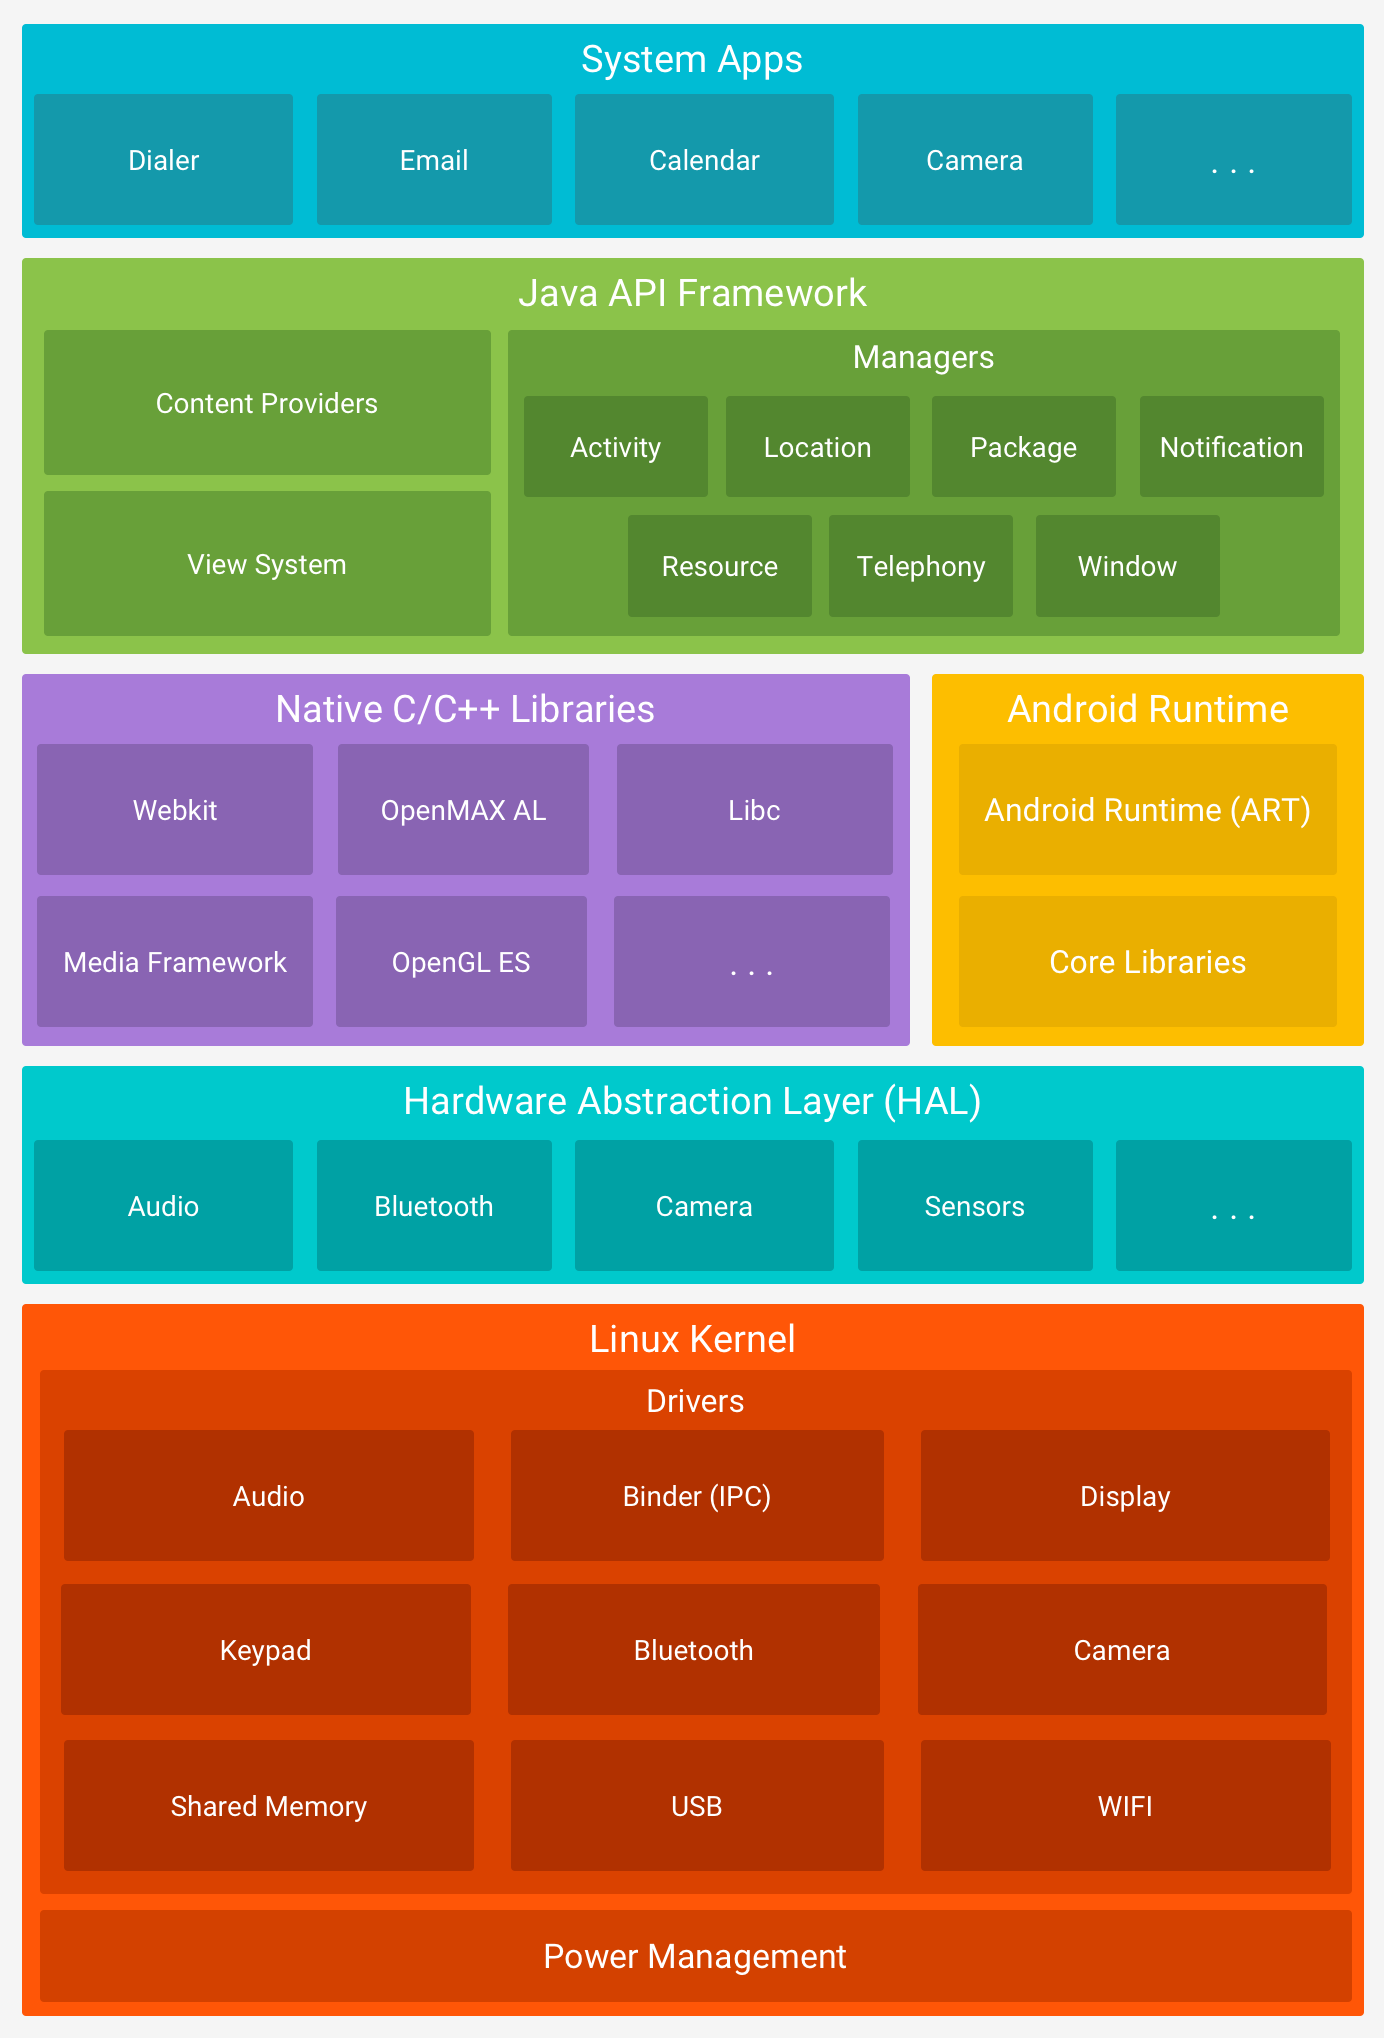
\includegraphics[width=0.9\textwidth, scale=0.9]{images/android}
	\caption{Android\label{fig:ALAP:sm2}}
\end{figure}

Az Android egy nyílt forráskódú, Linux kernel alapú többfelhasználós operációs rendszer, ahol minden applikáció egy külön felhasználó. Hivatalos nyelvei a Java és a Kotlin. Alapértelmezetten, a rendszer minden applikációnak kioszt egy egyedi Linux felhasználói ID-t (az ID-t csak a rendszer használja, és ismeretlen az applikáció számára). Az operációs rendszer úgy osztja ki a hozzáfárési jogokat az applikáció állományai számára, hogy csak az a felhasználói ID férjen hozzájuk, amivel az adott applikáció rendelkezik. Minden folyamat (process) rendelkezik a saját virtuális gépével, tehát minden applikáció kódja egymástól teljesen izoláltan fut. Alapértelmezetten minden applikáció a saját Linux folyamatában fut. Az Android operációs rendszer elindítja a folyamatot, amikor az applikáció valamelyik komponensének szüksége van rá, majd leállítja azt, mikor többé már nincs rá szükség, vagy ha a rendszernek mermóriát kell lefoglalnia, más applikációk számára. Az Android operációs rendszer “a legkevesebb kiváltság elvét” (“the principle of least privilige”) alkalmazza, tehát alapértelmezetten, minden applikációnak csak azokhoz a komponensekhez van hozzáférése, amik szükségesek a feladatának elvégzéséhez, és semmi egyébhez.

Egy android applikációnak négy fajta komponense lehet: Activity, Service, Broadcast receiver, Content provider. Ezek közül az Activity szolgál a felhasználóval történő interakció eszközéül, ez ugyanis egy felhasználói felülettel rendelkező képernyő. Activity-k, Service-k és Broadcast receiver-ek egy aszinkron üzenet által aktiválódnak, amit Intent-nek (szándék) nevezünk.

Az Activity egy osztály (class), amely a logikát tartalmazza, a felhasználói felületért azonban egy ehhez tartozó XML állomány felel, ami a különböző UI elemeket (gombok, szövegdobozok, konténerek) tartalmazza.

Az AndroidManifest.xml egy konfigurációs állomány, ami a projekt gyökér könyvtárában található. Itt vannak deklarálva az applikáció komponensei, valamint a szükséges hozzáférési jogokat is itt kell feltünteni.



The Linux Kernel
The foundation of the Android platform is the Linux kernel. For example, the Android Runtime (ART) relies on the Linux kernel for underlying functionalities such as threading and low-level memory management.

Using a Linux kernel allows Android to take advantage of key security features and allows device manufacturers to develop hardware drivers for a well-known kernel.

Hardware Abstraction Layer (HAL)
The hardware abstraction layer (HAL) provides standard interfaces that expose device hardware capabilities to the higher-level Java API framework. The HAL consists of multiple library modules, each of which implements an interface for a specific type of hardware component, such as the camera or bluetooth module. When a framework API makes a call to access device hardware, the Android system loads the library module for that hardware component.

Android Runtime
For devices running Android version 5.0 (API level 21) or higher, each app runs in its own process and with its own instance of the Android Runtime (ART). ART is written to run multiple virtual machines on low-memory devices by executing DEX files, a bytecode format designed specially for Android that's optimized for minimal memory footprint. Build toolchains, such as Jack, compile Java sources into DEX bytecode, which can run on the Android platform.

Some of the major features of ART include the following:

Ahead-of-time (AOT) and just-in-time (JIT) compilation
Optimized garbage collection (GC)
On Android 9 (API level 28) and higher, conversion of an app package's Dalvik Executable format (DEX) files to more compact machine code.
Better debugging support, including a dedicated sampling profiler, detailed diagnostic exceptions and crash reporting, and the ability to set watchpoints to monitor specific fields
Prior to Android version 5.0 (API level 21), Dalvik was the Android runtime. If your app runs well on ART, then it should work on Dalvik as well, but the reverse may not be true.

Android also includes a set of core runtime libraries that provide most of the functionality of the Java programming language, including some Java 8 language features, that the Java API framework uses.

Native C/C++ Libraries
Many core Android system components and services, such as ART and HAL, are built from native code that require native libraries written in C and C++. The Android platform provides Java framework APIs to expose the functionality of some of these native libraries to apps. For example, you can access OpenGL ES through the Android framework’s Java OpenGL API to add support for drawing and manipulating 2D and 3D graphics in your app.

If you are developing an app that requires C or C++ code, you can use the Android NDK to access some of these native platform libraries directly from your native code.

Java API Framework
The entire feature-set of the Android OS is available to you through APIs written in the Java language. These APIs form the building blocks you need to create Android apps by simplifying the reuse of core, modular system components and services, which include the following:

A rich and extensible View System you can use to build an app’s UI, including lists, grids, text boxes, buttons, and even an embeddable web browser
A Resource Manager, providing access to non-code resources such as localized strings, graphics, and layout files
A Notification Manager that enables all apps to display custom alerts in the status bar
An Activity Manager that manages the lifecycle of apps and provides a common navigation back stack
Content Providers that enable apps to access data from other apps, such as the Contacts app, or to share their own data
Developers have full access to the same framework APIs that Android system apps use.

System Apps
Android comes with a set of core apps for email, SMS messaging, calendars, internet browsing, contacts, and more. Apps included with the platform have no special status among the apps the user chooses to install. So a third-party app can become the user's default web browser, SMS messenger, or even the default keyboard (some exceptions apply, such as the system's Settings app).

The system apps function both as apps for users and to provide key capabilities that developers can access from their own app. For example, if your app would like to deliver an SMS message, you don't need to build that functionality yourself—you can instead invoke whichever SMS app is already installed to deliver a message to the recipient you specify.

%%%%%%%%%%%%%%%%%%%%%%%%%%%%%%%%%%%%%%%%%%%%%%%%%%%%%%%%%%%%%%%%%%%%%%%
\section{Gradle}\label{sec:ALAP:adatelem}

A Gradle egy nyílt forráskódú projektépítő eszköz (build automation tool). A Groovy, vagy Kotlin nyelvű scriptekbe, megadhatjuk a projektünk külső függöségeit (például API-k, library-k), melyeket letölti, majd lekompillálja és lefordítja a forráskódot.

Incremental Builds
Gradle checks in between build runs whether the input, output or an implementation of a task has changed since the last build invocation. If not, the task is considered up to date and is not executed. Gradle also considers the configuration of the task as part of its input.

Task Output Caching
If a task has already been executed on another computer, Gradle can skip the execution locally, and instead load the task's outputs from the build cache. The typical use case is to let CI builds push to a shared build cache, and allow developers to pull from it. A local build cache is also available to reuse task outputs produced earlier on the same machine.

Incremental Subtasks
When Gradle discovers that the input or output of a task has changed between build runs, the task is executed again. The task can use the incremental API to learn what files exactly have changed. With this information the task may not need to rebuild everything.

Compiler Daemon
When you need to fork the compilation process, Gradle creates a daemon process that is reused within a multi project build. This provides a dramatic speed improvement for the compilation process.

Parallel Execution
Gradle allows parallel execution of tasks and intra-task work through a Worker API. Parallelism is very fine-grained, resulting in faster performance.

Parallel Download of Dependencies
Gradle will download both dependency metadata (typically `pom.xml`) and artifacts in parallel. This is done on demand, only when the artifacts are actually required.


Android Applications
Official Android Build Tool
The Gradle Android Plugin and Android Studio are official tools provided and maintained by the Android SDK Tools team.

Android Domain Build Language
Describe your project via an Android-specific DSL. Tell Gradle about your project, now how to build it. Avoid the overly verbose need to explicitly implement the complex build process of Android projects.

Full Integration with Android Studio
Gradle is deeply integrated with Android Studio, the official Android IDE. In fact, Android Studio has no internal builder, it instead delegates all build tasks to Gradle. This "unified build system" ensures correctness across all your builds, whether they be run from Android Studio, the command line, or a continuous integration build server.

Build Variants
Declare your build types and product flavors and let Gradle handle the rest. No need to copy and paste build logic over and over for each of your project's variants. Use the expressive DSL to declare only what is different about your variants.

Android Library Projects
Android library projects are treated as first-class citizens in Gradle's multi-project build model. This enables all the benefits provided by Gradle's multi-project build support, such as project dependencies, and incremental builds.

Manifest Merging
Manifests and resource files are automatically merged, and individual entries overridden from variant source files. Build APKs with different application names, SKD versions or even required permissions.

Per-Variant Dependency Management
Gradle's advanced dependency management features are available to Android projects and can be configured uniquely for each build variant. Declare dependencies relevant to only certain variants or customize dependency resolution for each of your build variants.

Application Signing
Automate signing your applications. Debug build variants are, by default, signed with a debug key for installation on development devices. Declare additional signing configurations for publication to the Google Play store.

ProGuard Support
Easily configure ProGuard on your project to enable obfuscation and minification of the built APK. Configure ProGuard independently for each build type, allow an unoptimized APK for development and optimized one for release.

Unit Testing
Run unit tests against your Android application or library. Unit tests run in a standard Java JVM against a mocked Android SDK implementation facilitating fast-feedback test development, eliminating the overhead of building a separate APK and running tests of a device or emulator.

On-device Functional Testing
For tests that require a real Android environment for proper execution, bundle your test in a separate APK to be installed and run on an Android device or emulator. Separate APKs are built for each build variant allowing you to build and test every variant of your app in a single Gradle build.

APK Splits
Efficiently build multiple APKs for differing device display densities or ABIs by configuring Gradle to reuse shared build outputs.

Multidex Support
Utilize multidex support to avoid the 65k method limit imposed by Android DEX files.

NDK Support
Integrate your build with the Android NDK. Build application that depend on native libraries, projects that compile C/C++ into native libraries or both.

Databinding
Using binding classes generated by your Gradle build you can drastically simplify the way you interact with Android views. No more interacting with views directly, simply update the backing object and your view is kept up to date.

%%%%%%%%%%%%%%%%%%%%%%%%%%%%%%%%%%%%%%%%%%%%%%%%%%%%%%%%%%%%%%%%%%%%%%%
\section{Firebase}\label{sec:ALAP:szerkeszt}

A felhasználók adatainak, beállításainak tárolására, kezelésére a Firestore nevű no-sql (.json) alapú adatbázist használtam, mely a CRUD%
\footnote{ %
	create, read, update, delete
}  %
 műveletekhez is biztosít metódusokat. Logikai éptőelemei a kollekciók (collection) és a dokumentumok (document). Az előbbi tartalmazhat dokumentumokat, míg az utóbbi alkollekciókat, vagy magukat az adatokat. Az adatok kulcs, érték párok, az értékek lehetnek számok, karakterláncok, tömbök, geopontok vagy akár sajátos osztályok. Amennyiben sajátos osztály akarunk használni, annak rendelkeznie kell egy publikus konstruktorral, melynek nincsenek paraméterei, valamint az attribútumokhoz kell tartozzon egy-egy publikus „getter”%
 \footnote{ %
 	egy paraméter nélküli metódus, mely egy attribútumot térít vissza - példa: String getName()
 }  %
 metódus. Az adatbázisban található adatokhoz való hozzáférést egy szabállyal kell megadni, amelyet a szerver leellenőriz a CRUD műveletek végrehajtása esetén.

A felhasználók menedzselésére, mint a regisztráció, bejelentkezés, e-mail cím aktiválása, elfelejtett jelszó visszaállítása, a Firebase Authentication szolgáltatást használtam.



Users in Firebase Projects
A Firebase User object represents the account of a user who has signed up to an app in your Firebase project. Apps usually have many registered users, and every app in a Firebase project shares a user database.

A Firebase User instance is independent from a Firebase Auth instance. This means that you can have several references to different users within the same context and still call any of their methods.

User properties
A Firebase User has a fixed set of basic properties—a unique ID, a primary email address, a name and a photo URL—stored in the project's user database, that can be updated by the user (iOS, Android, web). You cannot add other properties to the Firebase User object directly; instead, you can store the additional properties in your Firebase Realtime Database.

The first time a user signs up to your app, the user's profile data is populated using the available information:

If the user signed up with an email address and password, only the primary email address property is populated
If the user signed up with a federated identity provider, such as Google or Facebook, the account information made available by the provider is used to populate the Firebase User's profile
If the user signed up with your custom auth system, you must explicitly add the information you want to the Firebase User's profile
Once a user account has been created, you can reload the user's information to incorporate any changes the user might have made on another device.

Sign-in providers
You can sign in users to your Firebase apps using several methods: email address and password, federated identity providers, and your custom auth system. You can associate more than one sign-in method with a user: for example, a user can sign in to the same account using an email address and a password, or using Google Sign-In.

A Firebase User instance keeps track of every provider linked to the user. This allows you to update empty profile's properties using the information given by a provider. See Managing Users (iOS, Android, web).

The current user
When a user signs up or signs in, that user becomes the current user of the Auth instance. The Firebase Auth instance persists the user's state, so that refreshing the page (in a browser) or restarting the application doesn't lose the user's information.

When the user signs out, the Auth instance stops keeping a reference to the User object and no longer persists its state; there is no current user. However, the user instance continues to be completely functional: if you keep a reference to it, you can still access and update the user's data.

The user lifecycle
The recommended way to track the current state of the Firebase Auth instance is by using listeners (also called "observers" in JavaScript). An Auth listener gets notified any time something relevant happens to the Auth object. See Managing Users (iOS, Android, web).

An Auth listener gets notified in the following situations:

The Auth object finishes initializing and a user was already signed in from a previous session, or has been redirected from an identity provider's sign-in flow
A user signs in (the current user is set)
A user signs out (the current user becomes null)
The current user's access token is refreshed. This case can happen in the following conditions:
The access token expires: this is a common situation. The refresh token is used to get a new valid set of tokens.
The user changes their password: Firebase issues new access and refresh tokens and renders the old tokens expired. This automatically expires the user's token and/or signs out the user on every device, for security reasons
The user re-authenticates: some actions require that the user's credentials are recently issued; such actions include deleting an account, setting a primary email address, and changing a password. Instead of signing out the user and then signing in the user again, get new credentials from the user, and pass the new credentials to the reauthenticate method of the User object.
Auth tokens
When you perform authentication with Firebase, there are three kinds of auth tokens you might encounter:

Firebase ID tokens	Created by Firebase when a user signs in to a Firebase app. These tokens are signed JWTs that securely identify a user in a Firebase project. These tokens contain basic profile information for a user, including the user's ID string, which is unique to the Firebase project. Because the integrity of ID tokens can be verified, you can send them to a backend server to identify the currently signed-in user.
Identity provider tokens	Created by federated identity providers, such as Google and Facebook. These tokens can have different formats, but are often OAuth 2.0 access tokens. Firebase apps use these tokens to verify that users have successfully authenticated with the identity provider, and then convert them into credentials usable by Firebase services.
Firebase custom tokens	Created by your custom auth system to allow users to sign in to a Firebase app using your auth system. Custom tokens are JWTs signed using a service account's private key. Firebase apps use these tokens much like they use the tokens returned from federated identity providers.



Cloud Firestore is a flexible, scalable database for mobile, web, and server development from Firebase and Google Cloud Platform. Like Firebase Realtime Database, it keeps your data in sync across client apps through realtime listeners and offers offline support for mobile and web so you can build responsive apps that work regardless of network latency or Internet connectivity. Cloud Firestore also offers seamless integration with other Firebase and Google Cloud Platform products, including Cloud Functions.

Cloud Firestore is currently in beta release. Feature availability and support for product integrations and platforms will continue to improve as the product matures. For more information on existing limitations in Cloud Firestore, see the limits and quotas documentation
GET STARTED

Key capabilities
Flexibility	The Cloud Firestore data model supports flexible, hierarchical data structures. Store your data in documents, organized into collections. Documents can contain complex nested objects in addition to subcollections.
Expressive querying	In Cloud Firestore, you can use queries to retrieve individual, specific documents or to retrieve all the documents in a collection that match your query parameters. Your queries can include multiple, chained filters and combine filtering and sorting. They're also indexed by default, so query performance is proportional to the size of your result set, not your data set.
Realtime updates	Like Realtime Database, Cloud Firestore uses data synchronization to update data on any connected device. However, it's also designed to make simple, one-time fetch queries efficiently.
Offline support	Cloud Firestore caches data that your app is actively using, so the app can write, read, listen to, and query data even if the device is offline. When the device comes back online, Cloud Firestore synchronizes any local changes back to Cloud Firestore.
Designed to scale	Cloud Firestore brings you the best of Google Cloud Platform's powerful infrastructure: automatic multi-region data replication, strong consistency guarantees, atomic batch operations, and real transaction support. We've designed Cloud Firestore to handle the toughest database workloads from the world's biggest apps.
How does it work?


Cloud Firestore is a cloud-hosted, NoSQL database that your iOS, Android, and web apps can access directly via native SDKs. Cloud Firestore is also available in native Node.js, Java, Python, and Go SDKs, in addition to REST and RPC APIs.

Following Cloud Firestore's NoSQL data model, you store data in documents that contain fields mapping to values. These documents are stored in collections, which are containers for your documents that you can use to organize your data and build queries. Documents support many different data types, from simple strings and numbers, to complex, nested objects. You can also create subcollections within documents and build hierarchical data structures that scale as your database grows. The Cloud Firestore data model supports whatever data structure works best for your app.

Additionally, querying in Cloud Firestore is expressive, efficient, and flexible. Create shallow queries to retrieve data at the document level without needing to retrieve the entire collection, or any nested subcollections. Add sorting, filtering, and limits to your queries or cursors to paginate your results. To keep data in your apps current, without retrieving your entire database each time an update happens, add realtime listeners. Adding realtime listeners to your app notifies you with a data snapshot whenever the data your client apps are listening to changes, retrieving only the new changes.

Protect access to your data in Cloud Firestore with Firebase Authentication and Cloud Firestore Security Rules for Android, iOS, and JavaScript, or Identity and Access Management (IAM) for server-side languages.

Implementation path
Integrate the Cloud Firestore SDKs	Quickly include clients via Gradle, CocoaPods, or a script include.
Secure your data	Use Cloud Firestore Security Rules or Identity and Access Management (IAM) to secure your data for mobile/web and server development, respectively.
Add Data	Create documents and collections in your database.
Get Data	Create queries or use realtime listeners to retrieve data from the database.

%%%%%%%%%%%%%%%%%%%%%%%%%%%%%%%%%%%%%%%%%%%%%%%%%%%%%%%%%%%%%%%%%%%%%%%
\section{Térkép}\label{sec:ALAP:szerkeszt}

\subsection{Distance Matrix API}

\subsection{Directions API}

A csomópontok közti távolságok mátrixának lekérdezésére a Distance Matrix API-t, valamint két csomópont közötti útvonal meghatározására a Directions API-t használtam.

The Distance Matrix API is a service that provides travel distance and time for a matrix of origins and destinations. The API returns information based on the recommended route between start and end points, as calculated by the Google Maps API, and consists of rows containing duration and distance values for each pair.


The Directions API is a service that calculates directions between locations using an HTTP request.

This video illustrates the use of the Directions API to help people find their way. The video includes advice on proxying the web service via your server when you're using the API in a mobile app, to protect your API key.


With the Directions API, you can:

Search for directions for several modes of transportation, including transit, driving, walking or cycling.
Return multi-part directions using a series of waypoints.
Specify origins, destinations, and waypoints as text strings (e.g. "Chicago, IL" or "Darwin, NT, Australia"), or as latitude/longitude coordinates, or as place IDs.
The API returns the most efficient routes when calculating directions. Travel time is the primary factor optimized, but the API may also take into account other factors such as distance, number of turns and many more when deciding which route is the most efficient.

Tip: Calculating directions is a time and resource intensive task. Whenever possible, use the service described here to calculate known addresses ahead of time and store the results in a temporary cache of your own design.

Note: This service is not designed to respond in real time to user input. For dynamic directions calculations (for example, within a user interface element), consult the documentation for the Maps JavaScript API Directions Service.
